\part{Backgroud and Related Work} \label{part:Background}
\chapter{Introduction to Cryptography} \label{ch:ItC}
Cryptology is the science of hiding and recovering secret information. It is mainly divided into two research areas: the areas of cryptography and cryptanalysis. Traditionally, cryptography is the study and practice of techniques that are used to establish secure communication between two parties in the presence of unauthorized third parties, usually called adversaries or attackers. Cryptography aims to prevent the adversary from learning anything about the original content of the communication, even if the adversary has some type of access to the communication channel. 

In general, if two parties would like to share some confidential information, they will share some secret information in advance. The piece of secret information will be used to transfer the original ordinary message (plaintext $P$) into an unintelligible message (ciphertext $C$) by the sender $S$. Additionally, $C$ can be transferred back to $P$ by the receiver $R$ using the same piece of secret information.  Formally, this secret information is called the key which is usually a short string of bits that needed to decrypt the ciphertext, while the transformations are called the encryption and decryption algorithms. 

Cryptanalysis is the sophisticated analysis and study of the security that a given cryptographic scheme offers. It focuses on the techniques related to recovering either the original content of an encrypted message without the knowledge of the secret key or some fraction of information from the message. This analysis is performed under different scenarios related to the adversary's resources, type of access, and the adversary's objectives. In general, the main purpose of cryptanalysis is to find the hidden weaknesses of a cryptosystem and develop a method of decryption.

In this chapter, we will give a brief introduction to two types of encryption systems: symmetric encryption systems and asymmetric encryption systems. We will discuss in detail block ciphers in symmetric cryptography, which are widely used and primarily implemented in the real world. 

\section{Symmetric and Asymmetric Encryptions}
Cryptographic algorithms are classified based on how key material is used and managed. Normally, they are classified into three groups. There are keyless algorithms, which do not use any key and do not need to trust anyone. Another type of algorithm uses a shared key, which needs to trust everyone that has the key.  The third type is private-public key algorithm, in which the private key is only known by one person \cite{PrCryEngCourtois}.
%They are normally classified as two groups. One group are keyless algorithms which do not use any key, such as hash functions. The other group is called cryptosystems which make use of key for encryption and decryption \cite{schneier1996applied}. Based on how the keys are managed, 

Generally, a cryptosystem has a sender $S$ and a receiver $R$ who want to send messages over an insecure channel. S and R are assumed to share a small amount of information beforehand, which is called the key. A cryptosystem is an encryption scheme that aims to protect the communication between S and R over an insecure channel.

A cryptosystem often contains an encryption function $E$, which takes a plaintext $p$ and a secret key $K$ which is composed of random bits and outputs a ciphertext $c = E_{K}(p)$, and the decryption function $D$ (inverse of $E$), which takes the ciphertext c and the secret key $K^{'}$ as input and recovers the initial plaintext, i.e. $D_{K^{'}}(c)=p$. The cryptosystem should be designed in such a way that even when adversaries obtain ciphertext, they cannot gain any information regarding the secret key or the plaintext.

In a cryptosystem, if $K = K^{'}$ which means the same secret key is used for both encryption and decryption, then the cryptosystem is called symmetric cryptosystem.

\begin{mydef}[Symmetric Cryptosystem]
	Let $P$ be the finite set of plaintexts, $C$ be the finite set of ciphertexts, and $K$ be the finite key space. An efficiently computable encryption function $E$ takes one plaintext in P and a key $k \in K$ returns a ciphertext in $C$. We write:  
	%A symmetric encryption scheme is a five-tuple ($P,C,K,\varepsilon, D$), where $P$ is the finite set of plaintext, $C$ is the finite set of ciphertext and $K$ is the key space such that $\forall k \in K$ there is an efficiently computable encryption function $E_{k} \in \varepsilon$ which respect to random bits k, 
	$$E_{k}:P \rightarrow C$$ 
	for the operation of executing $E$ on $k$ and $P$, and a corresponding efficiently computable decryption function is given by$D_{k}$: 
	$$ D_{k} : C \rightarrow P$$ 
	such that $D_{k}(E_{k}(p)) = p$ for all plaintext $p \in P$.
\end{mydef}

If the keys used for encryption and decryption are different to each other, but related in a way such that  decryption of a given ciphertext $c$ results in plaintext $p$, then the cryptosystem is called asymmetric cryptosystem.

\begin{mydef} [Asymmetric Cryptosystem]
	Let $P$ be the finite set of plaintexts, $C$ be the finite set of ciphertexts and $K$ be the key space. An efficiently computable key generation algorithm $keyGen()$ randomly generates a pair of public key $p_{k}$ and secret key $s_{k}$; an efficiently computable encryption function 
	$E$ takes one $p_{k} \in K$ and a plaintext in $P$ returns a cipher in $C$. We write: $$E_{p_{k}} : P \rightarrow C $$ and an $s_{k} \in K$ for the operation of executing $E$ on $p_{k}$ and P, and the corresponding efficiently computable decryption function is given by $D_{s_{k}} \in D$: $$ D_{s_{k}} : C \rightarrow P$$ such that $D_{s_{k}}(E_{p_{k}}(p)) = p $ for all plaintexts $p \in P$.
\end{mydef}
Note that symmetric cryptosystems have two algorithms: encryption and decryption. Asymmetric cryptosystems normally have at least three algorithms: key generation, encryption, and decryption. In a symmetric cryptosystem, if the key is compromised, then an adversary can decrypt any message passed from sender to receiver and gains full control over the system. Asymmetric cryptosystems solve this problem by using different, but corresponding keys, for encryption and decryption. However, modern cryptography sometimes requires a huge number of keys that must be distributed securely. 

Researchers start to solve the problem by combining both types of cryptosystem, called a $hybrid$ encryption scheme. This cryptosystem combines the convenience of asymmetric with the efficiency of a symmetric cryptosystem \cite{simmons1992contemporary}. In hybrid encryption, symmetric cryptosystem is used for encryption, while the secret key is shared using a protocol based on public-key cryptography, cf. \ref{hybird}. There are two main components of a hybrid encryption scheme, Key Encapsulation Mechanism (KEM) and Data Encapsulation Mechanism (DEM). The key feature is that the two parts are independent of one another. The framework was first formalized by Cramer and Shoup in 2003 and we refer the reader to \cite{cramer2003design} for more details.
\begin{figure}[h!]
	\centering
	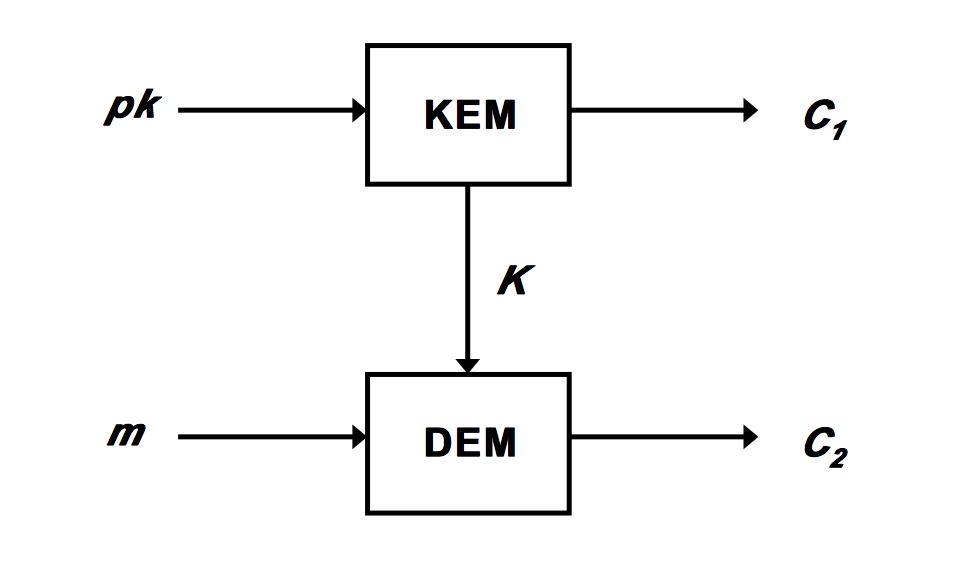
\includegraphics[width=80mm]{./pics/HybridEnc.png}
	\caption{Hybrid encryption}
	\label{hybird}
\end{figure}
\section{Block Ciphers}
A block cipher is a type of symmetric encryption system.  In block ciphers, the plaintext is divided into blocks of a fixed length, which are then encrypted into blocks of ciphertexts using the same key. Block ciphers are deterministic algorithms, which means that the same inputs result in the same outputs \cite{delfs2002introduction}. Block ciphers are considered as highly secure cryptography. Normally block ciphers are designed to be used for 50 years, while asymmetric cryptosystems are usually obsolete after 10 years (for example, NSA no longer recommends NIST P-256 elliptic curve in 2016\cite{NSA16}). 

The efficiently computable encryption algorithm $E_{K}(P)$ and decryption algorithm $D_{k}(C)$ in a block cipher both use blocks of $n$-bit as input and $k$-bit as a key $K$. $D_{k}(C)$ is the inverse of the encryption map $E_{K}(P)$. More formally, we have that: $$C = E_{K}(P) : \{0,1\}^{k} \times \{0,1\}^{n} \rightarrow \{0,1\}^{n}$$
$$D_{k}(C) = E_{K}^{-1}(P) : \{0,1\}^{k} \times \{0,1\}^{n} \rightarrow \{0,1\}^{n}$$
such that $D(E_{k}(P)) = P \quad  \forall K \in \{0,1\}^k$. 
%TO DO \forall and spaces

In general, for every key, a block cipher is a permutation of the form $\{0,1\}^{n} \rightarrow \{0,1\}^{n}$ for $n$-bit block. So in total there are $(2^{n}!) \simeq (2^{n-1})^{2^{n}}$ possible permutations. A block cipher which operates on $n$-bit blocks and uses $k$-bit keys is equivalent to a collection of $2^{k}$ distinct permutations on $n$-bit. A good design of a block cipher aims to choose the $2^{k}$ permutations uniformly at random\footnote{Or it is impossible to see if it was otherwise.} from the set of all $(2^{n}!)$ permutations.

Historical ciphers can be divided into three groups: substitution ciphers, transposition ciphers and product ciphers.
\subsection{Substitution Ciphers}
As indicated in the name, in substitution ciphers, every character in plaintext is substituted by some ciphertext character. There are four types of substitution ciphers: simple substitution, polyalphabetic substitution, homophonic substitution and polygram substitution \cite{knudsen1998block}. In this thesis, we only discuss simple and polyalphabetic substitutions:

\paragraph{Simple Substitution} \mbox{} \\ 
In a simple substitution cipher, each plaint text character is transformed into a ciphertext character via the same encryption function $E$. More formally, let $P = p_{0}, ... ,p_{n-1}$ be an $n$-character plaintext and $C=c_{0},...c_{n-1}$ be a ciphertext,  $\forall i : 0 \leq i < n $ 
$$ E : P \rightarrow C$$
$$c_{i} = f (p_{i})$$
%TODO: f is unbounded
Around 50 BC, Julius Caesar wrote to Marcus Cicero using a cipher that encrypted messages by shifting every letter in the plaintext three positions to the right in the alphabet. This cipher is based on \textit{shifted alphabets}. For the Caesar cipher, the secret key $k$ is $+3\mod{26}$. In general, the cipher is easily broken by shifting the ciphertexts one position until the plaintext arises.
\paragraph{Polyalphabetic Substitution} \mbox{} \\ 
In a polyalphabetic substitution, the characters in plaintext are transformed into ciphertext using a $j$-character key $K = k_{0}, k_{1}, ... k_{j-1}$, which defines j distinct encryption functions $E_{k_{0}}, E_{k_{1}}, ... , E_{k_{j-1}}$. In this case, $\forall i : 0 \leq i < n$  $$ E_{k_{l}} : P \rightarrow C   \qquad  \qquad   \forall l : 0 \leq l < j$$
$$ c_{i} = E_{k_{i\ mod\ j}}(p_{i})$$
The Vigen\`{e}re cipher \cite{robling1982cryptography}, first published in 1586, uses polyalphabetic substitution and is defined as follows:$$ c_{i} = E_{k_{i\ mod \ j}}(p_{i}) = p_{i} + k_{i\ mod \ j} $$
\subsection{Transposition Systems}
Transposition systems are essentially permutations of the characters in plaintext. Therefore, a transposition cipher is defined as follows $\forall i : 0 \leq i < n$ 
$$ \eta : \{0,...,(n-1)\} \rightarrow \{0,...,(n-1)\},\ a\ permutation$$
$$c_{i} = E(p_{i}) = p_{\eta (i)}$$
Many transposition ciphers operate by blocks which permute characters with a fixed period $j$. In that case:
$$ \eta : \{0,...,(j-1)\} \rightarrow \{0,...,(j-1)\},\ a\ permutation$$
$$c_{i} = E(p_{i}) = p_{(i\ div\ j)+\eta (i\ mod\ j)}$$
The Vigen\`{e}re and in general substitution ciphers can be broken when enough ciphertext is available to the cryptanalyst using the index of coincidence, Kasiski's method, etc. \cite{davies1989security,robling1982cryptography,kahn1996codebreakers}. Transposition ciphers can be broken using the frequency distributions for bigrams, trigrams, and $N$-grams \cite{davies1989security, robling1982cryptography, kahn1996codebreakers}. This knowledge about natural language is also very useful for our later work in password cracking.
\subsection{Product Ciphers}
To produce much stronger ciphers than the ones we have currently seen, we can combine substitution and transposition ciphers. These ciphers are called \textit{product ciphers}. Most block ciphers that are still used today are product ciphers. An iterated cipher is one kind of product ciphers in which the ciphertexts are computed by iteratively applying a round function several times to the plaintext. In each round, a round key is combined with the text input.
\begin{mydef}
	In an r-\textbf{round iterated block cipher}, the ciphertext is computed by iteratively applying a round function g to the plaintext, such that$$C_{i} = g(C_{i-1},K_{i}),\ i = 1,...,r$$ where $C_{0}$ is the plaintext, $K_{i}$ is a round key, and $C_{r}$ is the ciphertext. Decryption is done by reversing the above function. Therefore, for a fixed key $K_{i}$, $g$ must be invertible when $K_{i}$ is fixed.
\end{mydef}
\paragraph{Feistel Ciphers}\label{sec:feistel} \mbox{} \\
In general, it is not easy to make an invertible function that makes the encryption and decryption process identical. One method was created by the German physicist and cryptographer Horst Feistel, who was a pioneer in this area while working for American IBM. Feistel, together with Don Coppersmith, introduced the concept of Feistel networks while working on IBM's ``Lucifer'' cipher in 1973 \cite{feistel1973cryptography}. Their work gained the respect of the United States Federal Government who adapted it to the Data Encryption Standard (DES), which is based on the Lucifer project with some changes done by the NSA \cite{pub197746}.
\begin{figure}[h!]
	\centering
	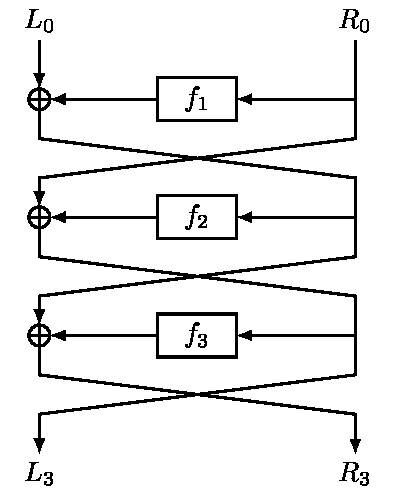
\includegraphics[width=80mm]{./pics/fofKW.png}
	\caption{Feistel network}
	\label{Fig:FeistelNet}
\end{figure}
\begin{mydef}	[Feistel Network, cf. Figure \ref{Fig:FeistelNet}]
A Feistel cipher is an iterated cipher that maps a 2t-bit plaintext block ($L_{0},R_{0}$) where $L_{0}$ and $ R_{0}$ are the left and right t-bit halves respectively, to a 2t-bit block ($L_{r}$,$R_{r}$) after r-rounds of encryption.
\end{mydef}
The result of $i$-rounds encryption $\forall i : 1 \leq i < r - 1 $ is computed as follows:
$$ L_{i} = R_{i-1}$$
$$ R_{i} = L_{i-1} \oplus f(R_{i-1},K_{i-1})$$
where $K_{i}$ is the $i$th subkey derived from the secret key $K$ and $f$ the one-round function which takes a subkey and a $t$-block as input to map into another $t$-bit block. This process is iteratively applied for $r - 2$ rounds. In the last round, there is no swap between two halves $L_{i-1}$ and $R_{i-1}$. This makes the decryption of the Feistel network the same as the encryption process, only requires a reversal of the key schedule. The final output is given by the following: $$ L_{r} = L_{r-1} \oplus f(R_{r-1},K_{r-1})$$
$$R_{r} = R_{r-1}$$

Since the encryption and decryption processes are identical (except for the key order), the software and hardware implementation of Feistel ciphers are much easier. 
\subsection{Courtois Toy Cipher}
